\documentclass{ximera}


\colorlet{regionColor}{black!30!white}
\begin{document}




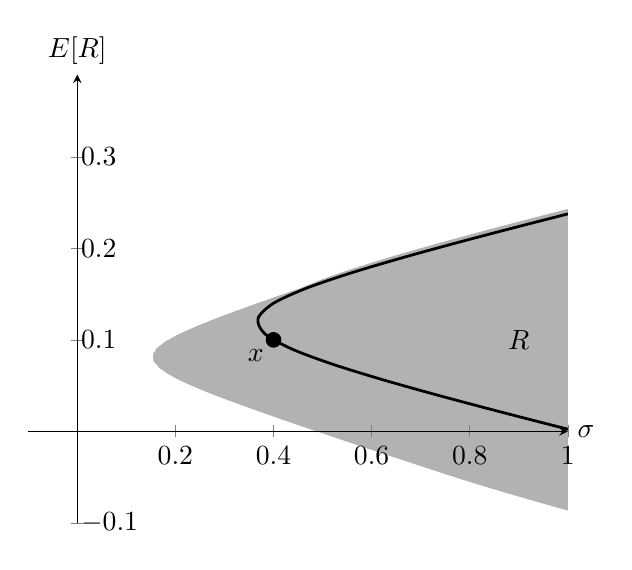
\begin{tikzpicture}
  \begin{axis}[
      xmin=-0.1,
      xmax=1,
      ymin=-0.1,
      ymax=.39,
      clip=true,
      %unit vector ratio*=1 1 1,
      axis lines=center,
      %grid = major,
      %ytick={-21,-18,...,21},
      %xtick={-21,-18,...,21},
      %ticks=none,
      xlabel=$\sigma$,
      ylabel=${E[R]}$,
      y tick label style={anchor=west},
      every axis y label/.style={at=(current axis.above origin),
        anchor=south},
      every axis x label/.style={at=(current axis.right of origin),anchor=west},
      axis on top,
    ]
    \foreach \u in {.55,.6,...,2}{
      \addplot[line width=1pt,
        regionColor,
        variable=\t,domain=-3:2,smooth] (
            {
              sqrt(.36-.96*\u-.6*\t+.9*\u*\t+.69*\u^2+.4*\t^2)
            },
            {
              .18-.14*\u-.08*\t
            });
            
    }

   \foreach \u in {-.1,-.05,...,1}{
      \addplot[line width=1pt,
        regionColor,
        variable=\t,domain=-2:3,smooth] (
            {
              sqrt(.36-.96*\u-.6*\t+.9*\u*\t+.69*\u^2+.4*\t^2)
            },
            {
              .18-.14*\u-.08*\t
            });
            
    }
    
    \addplot[draw=regionColor,fill=regionColor,fill opacity=1,domain=-1:1,mark=none,smooth] ({sqrt(1+140*x^2)-.84},{x+.08}) \closedcycle;
    \node at (axis cs: .9,.1) {$R$};

    \addplot[line width=1pt,
        black,
        variable=\t,domain=-2:3,smooth] (
            {
              sqrt(.36-.96*0-.6*\t+.9*0*\t+.69*0^2+.4*\t^2)
            },
            {
              .18-.14*0-.08*\t
            });
    \node[circle,fill,inner sep=2pt] at (axis cs:.4,.1) {};
    \node[below left] at (axis cs:.4,.1) {$x$};


  \end{axis}
\end{tikzpicture}














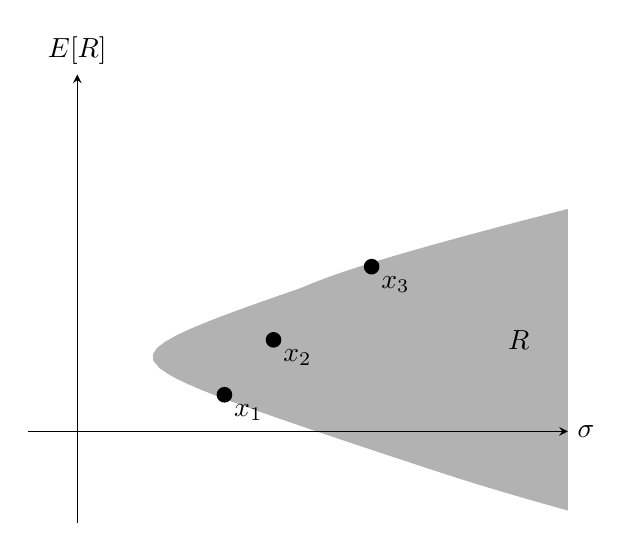
\begin{tikzpicture}
  \begin{axis}[
      xmin=-0.1,
      xmax=1,
      ymin=-0.1,
      ymax=.39,
      clip=true,
      %unit vector ratio*=1 1 1,
      axis lines=center,
      %grid = major,
      %ytick={-21,-18,...,21},
      %xtick={-21,-18,...,21},
      ticks=none,
      xlabel=$\sigma$,
      ylabel=${E[R]}$,
      y tick label style={anchor=west},
      every axis y label/.style={at=(current axis.above origin),
        anchor=south},
      every axis x label/.style={at=(current axis.right of origin),anchor=west},
      axis on top,
    ]
    \foreach \u in {.55,.6,...,2}{
      \addplot[line width=1pt,
        regionColor,
        variable=\t,domain=-3:2,smooth] (
            {
              sqrt(.36-.96*\u-.6*\t+.9*\u*\t+.69*\u^2+.4*\t^2)
            },
            {
              .18-.14*\u-.08*\t
            });
            
    }

   \foreach \u in {-.1,-.05,...,1}{
      \addplot[line width=1pt,
        regionColor,
        variable=\t,domain=-2:3,smooth] (
            {
              sqrt(.36-.96*\u-.6*\t+.9*\u*\t+.69*\u^2+.4*\t^2)
            },
            {
              .18-.14*\u-.08*\t
            });
            
    }
    
    \addplot[draw=regionColor,fill=regionColor,fill opacity=1,domain=-1:1,mark=none,smooth] ({sqrt(1+140*x^2)-.84},{x+.08}) \closedcycle;
    \node at (axis cs: .9,.1) {$R$};
    
    \node[circle,fill,inner sep=2pt] at (axis cs:.3,.04) {};
    \node[below right] at (axis cs:.3,.04) {$x_1$};

    \node[circle,fill,inner sep=2pt] at (axis cs:.4,.1) {};
    \node[below right] at (axis cs:.4,.1) {$x_2$};

    \node[circle,fill,inner sep=2pt] at (axis cs:.6,.18) {};
    \node[below right] at (axis cs:.6,.18) {$x_3$};


  \end{axis}
\end{tikzpicture}
\end{document}
